\documentclass[]{report}
\usepackage[margin=1.0in,top=1.5in]{geometry}
\usepackage{graphicx}
\usepackage{float}
\usepackage{hyperref}

% Title Page
\title{Pick-A-Tune}
\author{Phuc Pham, Samuel Oates, and Matthew Zelenin}

\begin{document}
\maketitle
\pagenumbering{Roman}
\renewcommand\thesection{\Roman{section}}
\renewcommand\thesubsection{\thesection.\arabic{subsection}}

\section{Challenges and Constraints}
	The objective of our project is to make a machine learning algorithm that takes songs as user input and returns back to the user recommendations of songs on Spotify based on their quantitative audio analysis.  Among our constraints on the problem space was limiting the number of songs users could input as well as the number of songs we would analyze from Spotify's database. We also had to narrow the amount of keywords used to make splits within the decision tree. Finally, we limited the number of songs we would return to the user.
	\subsection{Major Challenges}
	Some of the major challenges of the project came with understanding how various models of decision trees work and the construction of a functional decision tree. We had to look over the notes that were given to us in class and dig a bit more into researching the overall build of a decision tree. After our first check-in, we decided to ask our mentor for help on how the decision tree should be structure. They were able to provide us with links that were tremendously helpful to the design of the tree.  The first main problem that arose was how we would quickly and efficiently be able to obtain song data for any user-inputted song. At first, we tried to use MusicBrainz, an open music database, but the data was too large and it took over 20 minutes to look up a single song. We then had to search for a different database and eventually found the Spotify API which helped cut down the search run time.  Another major problem for us then became how to reformat our raw data so that it would be understood by the tree.  Then, there was a question of how we would test if the songs would be considered a recommended song for the user. Since this is more of a personal preference of the user, we had to use other means to test our songs. We decided to analyze the similarities of the artist, mood, beats, and other various attributes.
	\subsection{Variations}
	The variations that arose were how to design the decision tree and which database we could have used. As mentioned above, we were able to decide on the Spotify API being our database as it helped minimize the runtime of the overall algorithm, due to the constant number of songs it obtained through a quick search. We also did take a look at the previous project to see if we could use that implementation for our decision tree, but alas the assignment decision tree was highly confusing and Phuc could not seem to get the basics of it to use for our decision tree. Therefore, we asked the mentor for help; they provided us with links that ultimately helped create our current decision tree.
	
	\section{Machine Learning Task}  
	The machine learning task was to use the decision tree to correctly formulate a recommend playlist. We had to use multiple iterations of splitting the tree and analyze if each was the best split holistically, primarily due to the difficulty and ambiguity of trying to determine if two songs were similar. We tried to make it so that songs with similar mood and loudness would be grouped together and songs that had little connection with one another would be greatly distanced. Trying to accomplish this was challenging since the tree would often initially split on values that grouped the songs together that did not match one another. To make sure that the decision tree functioned correctly, we tried to use some of the training data on it. We started with five songs with very limited variance and we slowly increased the number of attributes that the decision tree could split on.
	
	\section{Algorithm \& Runtime}
	The algorithm that we chose was a decision tree. A decision tree is a decision support that structures itself like a tree and at every node of the tree, a decision is made to split the data. The decisions are made by calculating how many datapoints would be grouped together into two branches, usually true or false, of a node. As each node seeks to minimize the entropy of the dataset, measuring maximum information gain is used to determine which attributes should split the tree first. There are several ways to calculate information gain; in class, we learned to calculate the information gain using entropy, but after researching, we found that gini impurity seemed to produce a better runtime because it does not require logarithmic computation. Gini impurity is a measure of how often a randomly chosen element from the set would be incorrectly labeled if it was randomly labeled according to the distribution of labels in the subset. This can be computed by calculating the probability of the data multiplied by the probability of a miscalculation of that data.
	By using the decision tree with gini impurity, the runtime works out to about O(mn log n) where m is the number of attributes used; the partitioning of the branches then takes about O(n log n).
	\subsection{Limitations}
	We did not want to make the decision tree too complex because it would not generalize the training data well enough for the output. We also saw that if we made small changes upon the training data, this could cause the overall tree to change which would not make it robust.
	
	\section{Empirical Analysis}
	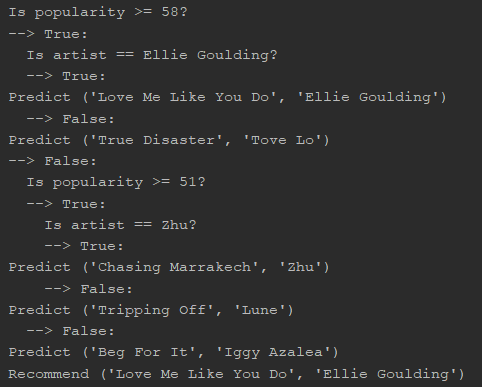
\includegraphics{FP1}
	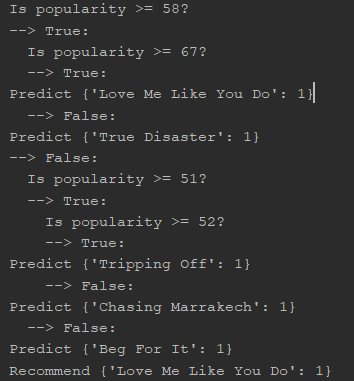
\includegraphics{FP2}
	The picture on the left is the result of our training data using artists as one of the attributes that would split the tree. The one on the right is the result of removing artists from the training data. We have decided to remove the artist since it would make splitting too precise. The other issue we hope to fix is that the decision tree algorithm sometimes recalls the same attribute multiple times to split the tree. This is not a result that we expected so we tried to correct it the best we could in our submission. This also implies that we need more attributes to help split the tree well.\\
	
	\begin{minipage}{0.5\textwidth}
		\begin{figure}[H]
			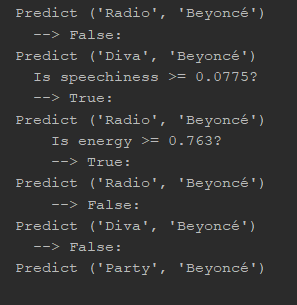
\includegraphics{decision_tree_at_work}
		\end{figure}
	\end{minipage} \hfill
	\begin{minipage}{0.45\textwidth}
			This is the final product of reworking the code. Sam was able to take in data produced by Matt and expanded the attributes that could be use to split the decision tree. The code does not reuse the same attribute to split the tree multiple time, which meant that the problem with the original iteration has been fixed.
	\end{minipage}

	\section{Outside Source Code}
	Firstly, the gini impurity was used to calculate the information gain that would be used to decide whether a split is good or not. It looks at how similar the data is in a list and give that list a value that is used to calculate the information gain values. This is made by Google Developer(\href{https://github.com/random-forests/tutorials/blob/master/decision\_tree.py}{Gini Source}). Then, our requests to Spotify's server for track and playlist information was done through a third-party service called Spotipy.  This module implements HTTP requests to fetch information from the server in easily called functions.  The module also allows for easy authentication, linking our Spotify Developers profile and application to our Python code.  While we analyzed the source code responsible for delivering the server requests to understand how it worked, we elected to use this third-party software in order to more directly tackle the machine learning aspects of our project and its general correlation with class material.
	
	\section{Improvements?}
	To improve the AI, we should have implemented a decision tree with pruning to compare how well it would have worked with our based data and advance the type of splits that we are making. We would have liked to do further research to see if gini impurity is in fact the fastest way to calculate information gain or if a better computational function could be used. Gini impurity was only slightly more efficiently than calculating entropy, leading us to believe there is in fact a more efficient computation. Sam and Matt specifically enjoyed learning how to use the Spotify API to clean the data to a point where they were able to get an abundance testing and training.
\end{document}          
